\documentclass[15pt]{report}
%\usepackage[utf8]{inputenc}
\usepackage{graphicx}
\usepackage{fancyhdr}
\pagestyle{fancy}
\usepackage{amssymb}
\usepackage{bbm}
\graphicspath{ {images/} }
\usepackage[backend=bibtex]{biblatex}
\usepackage{graphicx}

\usepackage{listings}
\usepackage{color}

\definecolor{dkgreen}{rgb}{0,0.6,0}
\definecolor{gray}{rgb}{0.5,0.5,0.5}
\definecolor{mauve}{rgb}{0.58,0,0.82}

\lstset{frame=tb,
  language=Python,
  aboveskip=3mm,
  belowskip=3mm,
  showstringspaces=false,
  columns=flexible,
  basicstyle={\small\ttfamily},
  numbers=none,
  numberstyle=\tiny\color{gray},
  keywordstyle=\color{blue},
  commentstyle=\color{dkgreen},
  stringstyle=\color{mauve},
  breaklines=true,
  breakatwhitespace=true,
  tabsize=3
}
\lstnewenvironment{code}%
  {\noindent\minipage{\linewidth}
   \lstset{}}
  {\endminipage}


\renewcommand*{\arraystretch}{1.5}

\newcommand{\dx}[1]{ \frac{\partial}{\partial x^{#1} }}
\newcommand{\dxx}[2]{ \frac{\partial x^{#1}}{\partial x^{#2} }}

%\bibliography{ref1}
\setcounter{tocdepth}{3}
\title{PyGravity \\
		\small http://github.com/russloewe/PyGravity}

\author{Russell Loewe}

\date{7~May 2015}

\begin{document}

\maketitle

\indent
This is the supporting documentation for
\textit{PyGravity} 

\tableofcontents
% \setcounter{section}{-1}

\newpage
\chapter{Foreward}

\section{About}

\paragraph{}PyGravity is a gravity simulating tool written in Python. PyGravity's purpose is to be able to take an arbitrary 
of objects  from small particles to large bodies such as planets or stars and calculate the progression of their movements 
in an arbitrary number of dimensions. The main focus on this project is precision of calculations and not on speed. This program 
will quickly hit very long run times with even small data sets. 
\paragraph{}PyGravity is not for real time calculations. The aim is to take an input file that contains the position, mass, and 
velocities of objects in a system and output the evolution of the system to a high degree of precision. The outputted data can be 
either directly graphed with graphing software such as Matplotlib, or saved to a CSV file where it can later either be graphed, 
animated or plugged back into PyGravity for further calculations.

\section{Features}
\paragraph{Arbitrary Dimension} PyGravity defaults to 3 spatial dimensions, but it can easily be configured to work in any 
number of spatial dimensions. The underlying code treats all vectors as having arbitrary dimension. As long as the dimension 
of the vectors match any calculation can be performed, from norming vectors, finding distances, or calculating and applying forces. 
There is currently a dimensions attribute on the base package. Usage is outlined in the next chapter, but it's existence is 
strictly for the CSV parser when loading object from a file. This is even just a stand in until a smarter parser is created.

\paragraph{Precision}The precision is carried out by Python's Decimal module. The precision is defaulted to 200 but can be 
adjusted for either greater accuracy or greater speed.

\paragraph{Vector Physics} There are a number of vector physics employed in PyGravity that are accessible independently. Some 
examples are getting directional and unit vectors between two locations, finding the force of gravity in a system of many objects, 
finding the escape velocity for each individual object in a system of many.

\section{Maintainer}
\paragraph{} Latest code is on github at \textit{http://github.com/russloewe/PyGravity} . Issues can be directly emailed to the 
maintainer at russloewe@gmail.com . 

\chapter{Examples}
\section{4 Body Circular Orbit}
\paragraph{}Starting the examples with one of my favourites, let's simulated a ring of planets. In this example each planet, or 
asteroid, will have equal mass, start off in a ring, with initial velocities pointing pointing in a circle. This is illustrated 
in the below graphic. The black arrows indicate the initial velocity of each object. The positions and velocities are defined in
 example\_data.csv .

\centerline{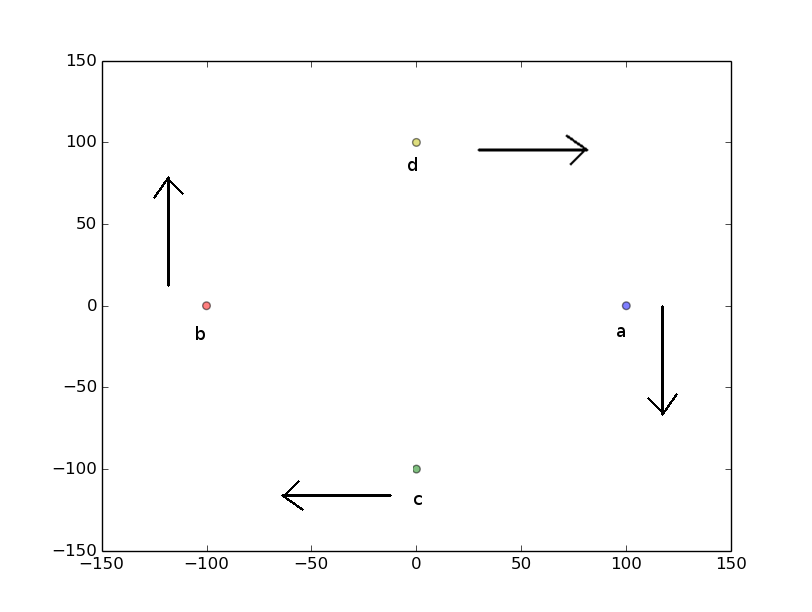
\includegraphics[scale=0.5]{./img/ex1_0}}

\paragraph{exmple\_data}


\begin{code}
a:100:0:0:0:-0.09:0:1.55e10
b:-100:0:0:0:0.09:0:1.55e10
c:0:-100:0:-0.09:0:0:1.55e10
d:0:100:0:0.09:0:0:1.55e10
\end{code}

\paragraph{code}

\begin{code}
import numpy as np
import matplotlib.pyplot as plt
import PyGravity

# Created base instance for PyGravity
base = PyGravity.PyGravity()

# Set spatial dimension, not required, default is 3  
base.dimension = 3

# Load data from data file
base.read_file('example_data.csv')

# Set time step to 60 seconds (1 minute)
base.Physics.timestep = 60

# lower precision to 100, from default of 200
base.Physics.prec = 100

# create empty lists for each objects x and y position
# ignore z since all z values are zero
ax = []
ay = []
bx = []
by = []
cx = []
cy = []
dx = []
dy = []

# save each objects location into the above lists  for each timestep, or in this case for 
# each minute
for i in range(10):
    ax.append(base.Physics.objects[0].P[0])
    ay.append(base.Physics.objects[0].P[1])
    bx.append(base.Physics.objects[1].P[0])
    by.append(base.Physics.objects[1].P[1])
    cx.append(base.Physics.objects[2].P[0])
    cy.append(base.Physics.objects[2].P[1])
    dx.append(base.Physics.objects[3].P[0])
    dy.append(base.Physics.objects[3].P[1])

	# calculate the positions of each object for the next time interval (minute)
    base.Physics.step_all()
   
# add each data list to the graph
plt.scatter(ax, ay, s=10, c='b', alpha=0.5)
plt.scatter(bx, by, s=10, c='r', alpha=0.5)
plt.scatter(cx, cy, s=10, c='g', alpha=0.5)
plt.scatter(dx, dy, s=10, c='y', alpha=0.5)
plt.show()

\end{code}

\paragraph{10 min}
\centerline{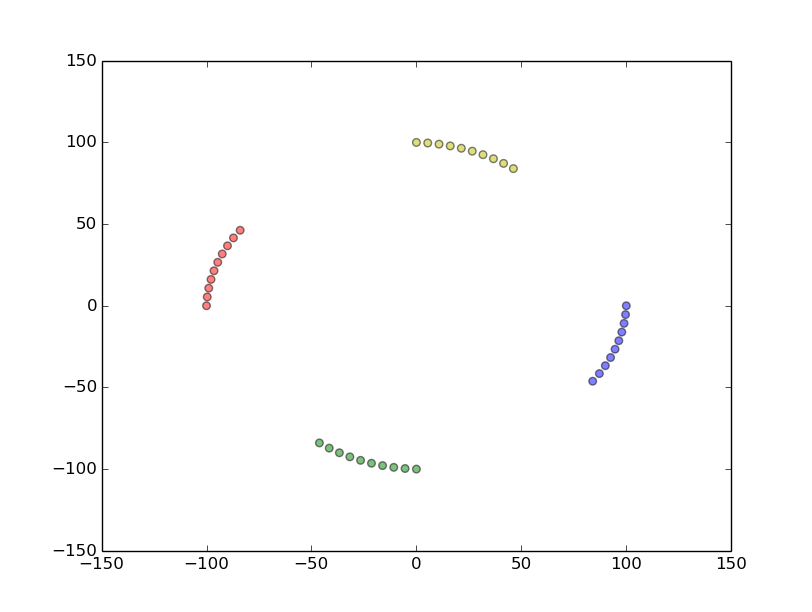
\includegraphics[scale=0.3]{./img/ex1_1}}

\paragraph{20 min}
\centerline{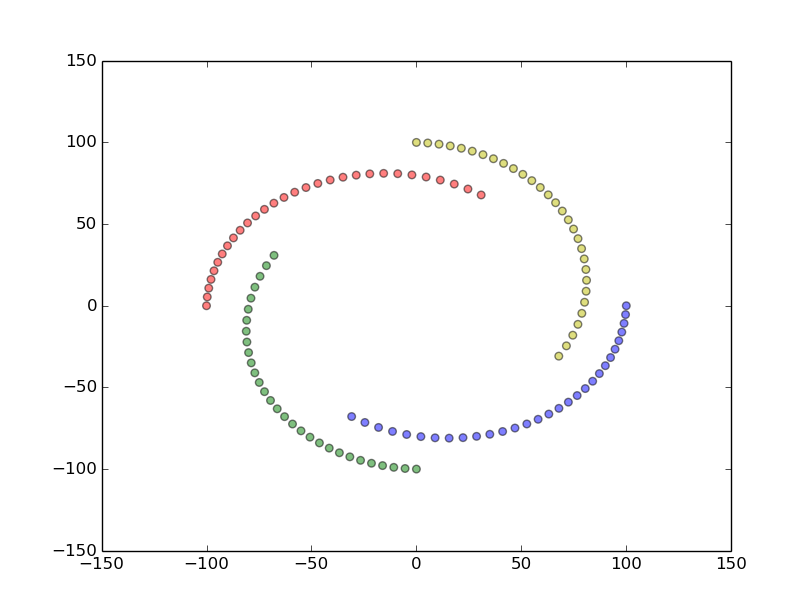
\includegraphics[scale=0.3]{./img/ex1_2}}

\paragraph{90 min}
\centerline{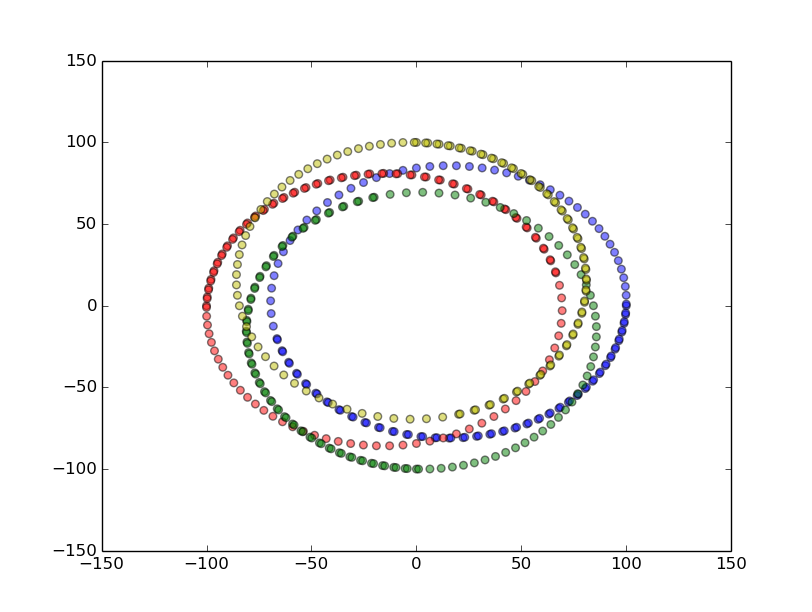
\includegraphics[scale=0.3]{./img/ex1_3}}



\end{document}
